%%% File-Information {{{
%%% Filename: template_bericht.tex
%%% Purpose: lab report, technical report, project report
%%% Time-stamp: <2004-06-30 18:19:32 mp>
%%% Authors: The LaTeX@TUG-Team [http://latex.tugraz.at/]:
%%%          Karl Voit (vk), Michael Prokop (mp), Stefan Sollerer (ss)
%%% History:
%%%   20040630 (mp) added comments to foldmethod at end of file
%%%   20040625 (vk,ss) initial version
%%%
%%% Notes:
%%%
%%%
%%%
%%% }}}
%%%%%%%%%%%%%%%%%%%%%%%%%%%%%%%%%%%%%%%%%%%%%%%%%%%%%%%%%%%%%%%%%%%%%%%%%%%%%%%%
%%% main document {{{

\documentclass[
a4paper,     %% defines the paper size: a4paper (default), a5paper, letterpaper, ...
% landscape,   %% sets the orientation to landscape
% twoside,     %% changes to a two-page-layout (alternatively: oneside)
% twocolumn,   %% changes to a two-column-layout
headsepline, %% add a horizontal line below the column title
footsepline, %% add a horizontal line above the page footer
titlepage,   %% only the titlepage (using titlepage-environment) appears on the first page (alternatively: notitlepage)
halfparskip,     %% insert an empty line between two paragraphs (alternatively: halfparskip, ...)
% leqno,       %% equation numbers left (instead of right)
% fleqn,       %% equation left-justified (instead of centered)
% tablecaptionabove, %% captions of tables are above the tables (alternatively: tablecaptionbelow)
%draft,       %% produce only a draft version (mark lines that need manual edition and don't show graphics)
% 10pt         %% set default font size to 10 point
12pt,         %% set default font size to 11 point
DIV16
]{scrartcl}  %% article, see KOMA documentation (scrguide.dvi)

%%%%%%%%%%%%%%%%%%%%%%%%%%%%%%%%%%%%%%%%%%%%%%%%%%%%%%%%%%%%%%%%%%%%%%%%%%%%%%%%
%%%
%%% packages
%%%

%%%
%%% encoding and language set
%%%

%%% ngerman: language set to new-german
\usepackage{ngerman}

%%% inputenc: coding of german special characters
\usepackage[latin1]{inputenc}

%%% fontenc, ae, aecompl: coding of characters in PDF documents
\usepackage[T1]{fontenc}
\usepackage{ae,aecompl}

%%%
%%% technical packages
%%%

%%% amsmath, amssymb, amstext: support for mathematics
\usepackage{amsmath,amssymb,amstext}

%%% psfrag: replace PostScript fonts
\usepackage{psfrag}

%%% listings: include programming code
\usepackage{listings}
\usepackage{moreverb}

%%% units: technical units
\usepackage{units}

%%% color: support for ... colors, yes!
\usepackage{color}

%%% pstricks, pst-uml: UML diagrams
\usepackage{pstricks}
\usepackage{pst-uml}

%%% table-stuff
\usepackage{booktabs}
%\usepackage{array}
%\usepackage{multirow}

%\newcolumntype{N}{>{\bfseries\scriptsize}l}
%\newcolumntype{V}[1]{%
	%>{\bfseries\scriptsize\raggedright\hspace{0pt}}p{#1}%
%}

%%% dbicons: ERM
\usepackage{dbicons}

%%% some color-definitions (see http://texnik.de/listings/listing0.pdf)
\definecolor{hellgelb}{rgb}{1,1,0.8}
\definecolor{hellgrau}{rgb}{0.9,0.9,0.9}
\definecolor{colKeys}{rgb}{0,0,1}
\definecolor{colIdentifier}{rgb}{0,0,0}
\definecolor{colComments}{rgb}{1,0,0}
\definecolor{colString}{rgb}{0,0.5,0}

%%% configuration of the listings-package
\lstset{%
	float=hbp,%
	basicstyle=\ttfamily\footnotesize, %
	identifierstyle=\color{colIdentifier}, %
	keywordstyle=\color{colKeys}, %
	stringstyle=\color{colString}, %
	commentstyle=\color{colComments}, %
	columns=flexible, %
	tabsize=4, %
	frame=tb, %
	extendedchars=true, %
	showspaces=false, %
	showstringspaces=false, % 
	numbers=left, %
	numberstyle=\tiny, %
	breaklines=true, %
	backgroundcolor=\color{hellgrau}, %
	breakautoindent=true, %
	captionpos=b%
}

%%%
%%% layout
%%%

%%% scrpage2: KOMA heading and footer
%%% Note: if you don't use this package, please remove 
%%%       \pagestyle{scrheadings} and corresponding settings
%%%       below too.
\usepackage{scrpage2}

% EM unterstrichen darstellen
\usepackage{ulem}

% Schrift fuer Captions verkleinern
%\setkomafont{captionlabel}{\scriptsize}
%\setkomafont{caption}{\usekomafont{captionlabel}}

% Float
\usepackage{float}

%%%
%%% PDF
%%%

\newif\ifpdf
  \ifx\pdfoutput\undefined
     \pdffalse
  \else
     \pdfoutput=1
     \pdftrue
  \fi

%%% Should be LAST usepackage-call!
%%% For docu on that, see reference on package ``hyperref''
\ifpdf{%   (definitions for using pdflatex instead of latex)

	%%% for screen (PDF), we use sans-serif-fonts
	\usepackage{mathpazo}
	\usepackage[scaled=.95]{helvet}
	\usepackage{courier}	
	\renewcommand{\familydefault}{\sfdefault}
	\usepackage[sf]{titlesec}

  %%% graphicx: support for graphics
  \usepackage[pdftex]{graphicx}
 
  \pdfcompresslevel=9

  %%% hyperref (hyperlinks in PDF): for more options or more detailed
  %%%          explanations, see the documentation of the hyperref-package
  \usepackage[%
    %%% general options
    pdftex=true,      %% sets up hyperref for use with the pdftex program
    %plainpages=false, %% set it to false, if pdflatex complains: ``destination with same identifier already exists''
    %
    %%% extension options
    backref=section,   %% if true, adds a backlink text to the end of each item in the bibliography
    pagebackref=false, %% if true, creates backward references as a list of page numbers in the bibliography
    colorlinks=true,   %% turn on colored links (true is better for on-screen reading, false is better for printout versions)
    %
    %%% PDF-specific display options
    bookmarks=true,          %% if true, generate PDF bookmarks (requires two passes of pdflatex)
    bookmarksopen=false,     %% if true, show all PDF bookmarks expanded
    bookmarksnumbered=false, %% if true, add the section numbers to the bookmarks
    %pdfstartpage={1},        %% determines, on which page the PDF file is opened
    pdfpagemode=None,	       %% None, UseOutlines (=show bookmarks), UseThumbs (show thumbnails), FullScreen
    breaklinks=true         
  ]{hyperref}


  %%% provide all graphics (also) in this format, so you don't have
  %%% to add the file extensions to the \includegraphics-command
  %%% and/or you don't have to distinguish between generating
  %%% dvi/ps (through latex) and pdf (through pdflatex)
  \DeclareGraphicsExtensions{.pdf}
  \graphicspath{{./images}}

\else    %(definitions for using latex instead of pdflatex)

  \usepackage[dvips]{graphicx}

  \DeclareGraphicsExtensions{.eps}
  \graphicspath{{./images}}  

  \usepackage[%
    dvips,            %% sets up hyperref for use with the dvips driver
    colorlinks=false, %% better for printout version; almost every hyperref-extension is eliminated by using dvips
    breaklinks=true 
  ]{hyperref}

\fi %ifpdf

%%% sets the PDF-Information options
%%% (see fields in Acrobat Reader: ``File -> Document properties -> Summary'')
%%% Note: this method is better than as options of the hyperref-package (options are expanded correctly)
\hypersetup{
  pdftitle={Informationssystem zur Verwaltung und Buchung von Ferienwohnungen �ber Internet (IVBF)}, %%
  pdfauthor={Jan Tammen <foobar@fh-konstanz.de>}, %%
  pdfsubject={Datenbanksysteme, 1. Praktikumsabschnitt}, %%
  pdfcreator={Jan Tammen <foobar@fh-konstanz.de>}, %% 
  pdfproducer={}, %%
  pdfkeywords={} %%
}


%%%%%%%%%%%%%%%%%%%%%%%%%%%%%%%%%%%%%%%%%%%%%%%%%%%%%%%%%%%%%%%%%%%%%%%%%%%%%%%%
%%%
%%% user defined commands
%%%

%%% \mygraphics{}{}{}
%% usage:   \mygraphics{width}{filename_without_extension}{caption}
%% example: \mygraphics{0.7\textwidth}{rolling_grandma}{This is my grandmother on inlinescates}
%% requires: package graphicx
%% provides: including centered pictures/graphics with a boldfaced caption below
%% 
\newcommand{\mygraphics}[3]{
  \begin{center}
    \includegraphics[width=#1, keepaspectratio=true]{#2} \\
    \textbf{#3}
  \end{center}
}

%%%%%%%%%%%%%%%%%%%%%%%%%%%%%%%%%%%%%%%%%%%%%%%%%%%%%%%%%%%%%%%%%%%%%%%%%%%%%%%%
%%%
%%% define the titlepage
%%%

% \subject{}   %% subject which appears above titlehead
% \titlehead{} %% special heading for the titlepage

%%% title
\title{Informationssystem zur Verwaltung und Buchung von Ferienwohnungen �ber Internet (IVBF)}
\subject{Datenbanksysteme, 1. Praktikumsabschnitt}

%%% author(s)
\author{Jan Tammen \href{mailto:foobar@fh-konstanz.de}{<foobar@fh-konstanz.de>}}

%\publishers{Ort der Durchf�hrung: EDC-Labor, FH Konstanz.\\
%						Datum: 16.12.2004}

\date{\today}

% \thanks{} %% use it instead of footnotes (only on titlepage)

% \dedication{} %% generates a dedication-page after titlepage

%%%%%%%%%%%%%%%%%%%%%%%%%%%%%%%%%%%%%%%%%%%%%%%%%%%%%%%%%%%%%%%%%%%%%%%%%%%%%%%%
%%%
%%% set heading and footer
%%%

%%% scrheadings default: 
%%%      footer - middle: page number
\pagestyle{scrheadings}

%%% user specific
%%% usage:
%%% \position[heading/footer for the titlepage]{heading/footer for the rest of the document}

%%% heading - left
% \ihead[]{}

%%% heading - center
% \chead[]{}

%%% heading - right
% \ohead[]{}

%%% footer - left
% \ifoot[]{}

%%% footer - center
% \cfoot[]{}

%%% footer - right
% \ofoot[]{}



%%%%%%%%%%%%%%%%%%%%%%%%%%%%%%%%%%%%%%%%%%%%%%%%%%%%%%%%%%%%%%%%%%%%%%%%%%%%%%%%
%%%
%%% begin document
%%%
\setcounter{section}{-1}
\begin{document}

% \pagenumbering{roman} %% small roman page numbers

%%% include the title
%\thispagestyle{empty}  %% no header/footer (only) on this page
\maketitle

%%% start a new page and display the table of contents
\newpage
\tableofcontents

%%% start a new page and display the list of figures
%\newpage
%\listoffigures

%%% start a new page and display the list of tables
% \newpage
% \listoftables

%%% display the main document on a new page 
\newpage

% \pagenumbering{arabic} %% normal page numbers (include it, if roman was used above)

%%%%%%%%%%%%%%%%%%%%%%%%%%%%%%%%%%%%%%%%%%%%%%%%%%%%%%%%%%%%%%%%%%%%%%%%%%%%%%%%
%%%
%%% begin main document
%%% structure: \section \subsection \subsubsection \paragraph \subparagraph
%%%

\section{Einleitung}
Es soll ein Internet-System entwickelt werden, welches Interessenten das Abrufen von
Informationen �ber Ferienwohnungen erm�glicht sowie Buchungen von Wohnungen durch registrierte Kunden 
aufnimmt und verwaltet.

\section{Konzeptioneller Entwurf}
\subsection{Systemanforderungen}
Die an das System gestellten Anforderungen enthalten die folgenden Abl�ufe und Daten:

\begin{itemize}
	\item Speicherung von Ferienwohnungen mit Angaben: Zuordnung zu einem Land, Anzahl Zimmer, Gr��e, Preis/Tag,
				hat die W. eine Sauna?, hat die W. ein Schwimmbad?, bis zu vier Bilder
	\item Speicherung von Touristenattraktionen mit Angaben: Zuordnung zu einem Land, Typ 
				(z.B. "`Freizeitpark"') und Name
	\item Speicherung der Entfernung zwischen einzelnen Ferienwohnung und Attraktionen
	\item Speicherung von Fluglinien mit Name sowie eine Zuordnung zu angeflogenen L�ndern
	\item Abrufen von Informationen �ber eine Wohnung durch einen Interessenten, Anzeige aller Informationen, suchen
				nach speziellen Kriterien
	\item Registrierung, dadurch Erreichen des "`Kunden"'-Status
	\item Speicherung von Kundendaten: Name, Adresse, Zuordnung zu Land, Bankverbindung
	\item Buchung einer Ferienwohnung f�r einen speziellen Zeitraum durch registrierte Kunden
	\item Nach erfolgreicher Buchung: Erstellung einer Rechnung mit eindeutiger Buchungsnummer. Nach Zahlungseingang:
				Speicherung des Datums des Zahlungseinganges.
\end{itemize}

Aus diesen Anforderungen l�sst sich das im folgenden Abschnitt aufgef�hrte UML Use-Case-Diagramm erstellen.

\subsubsection{Anwendungsf�lle}

\begin{figure}[H]
	\centering
		\input usecasediag
	\caption{Use-Case-Diagramm}
	\label{fig:usecasediag}
\end{figure}

\subsection{Layout einiger Internetseiten}
Die Interaktion mit dem Systembenutzer erfolgt �ber Eingabemasken, zu deren
Illustration hier einige schematische Beispiele aufgef�hrt sind.

\subsubsection{Suche nach einer Ferienwohnung}
\begin{figure}[H]
	\centering
		\includegraphics[width=0.80\textwidth]{images/screen_suche.eps}
	\caption{Layoutbeispiel: Suche nach einer Ferienwohnung}
	\label{fig:screen_suche}
\end{figure}

\subsubsection{Anzeige der Suchergebnisse}
\begin{figure}[H]
	\centering
		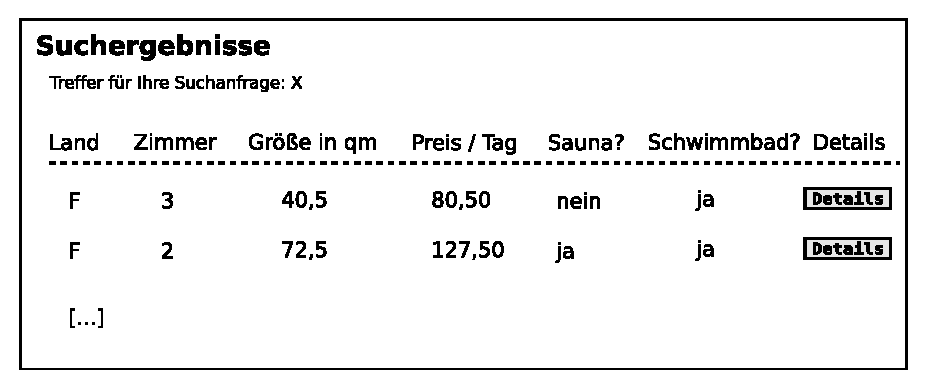
\includegraphics[width=0.75\textwidth]{images/screen_ergebnisse.eps}
	\caption{Layoutbeispiel: Anzeige der Suchergebnisse}
	\label{fig:screen_ergebnisse}
\end{figure}

\subsubsection{Detailansicht einer Ferienwohnung}
\begin{figure}[H]
	\centering
		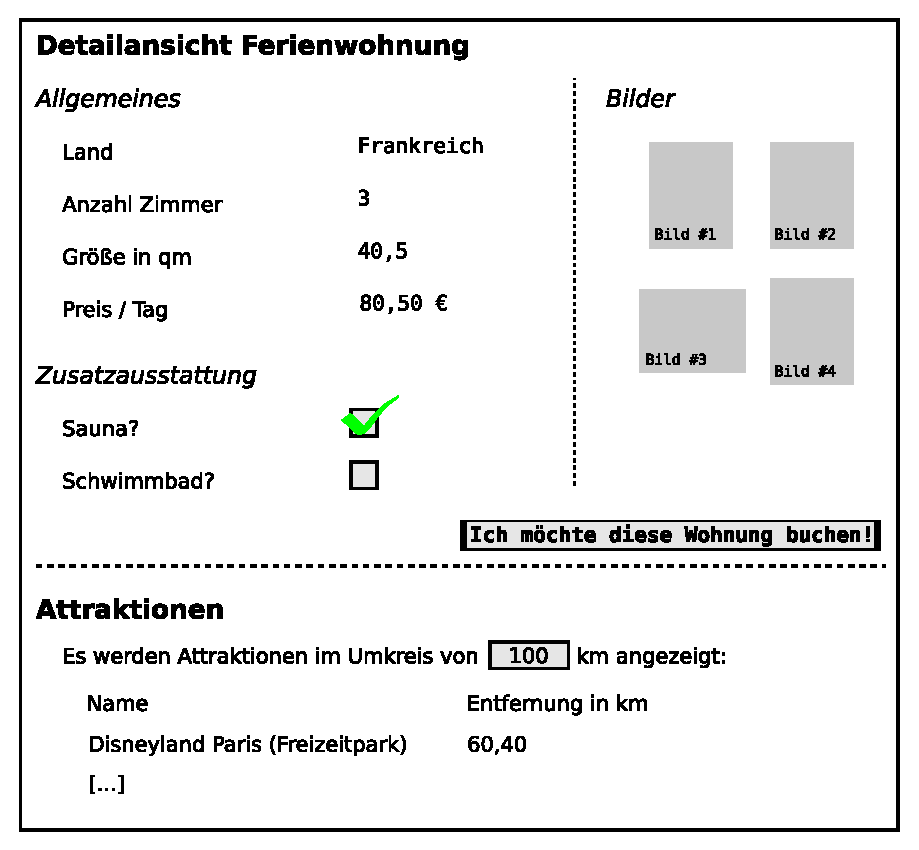
\includegraphics[width=0.70\textwidth]{images/screen_detail.eps}
	\caption{Layoutbeispiel: Detailansicht einer Ferienwohnung}
	\label{fig:screen_detail}
\end{figure}

\subsubsection{Buchung einer Ferienwohnung}
\begin{figure}[H]
	\centering
		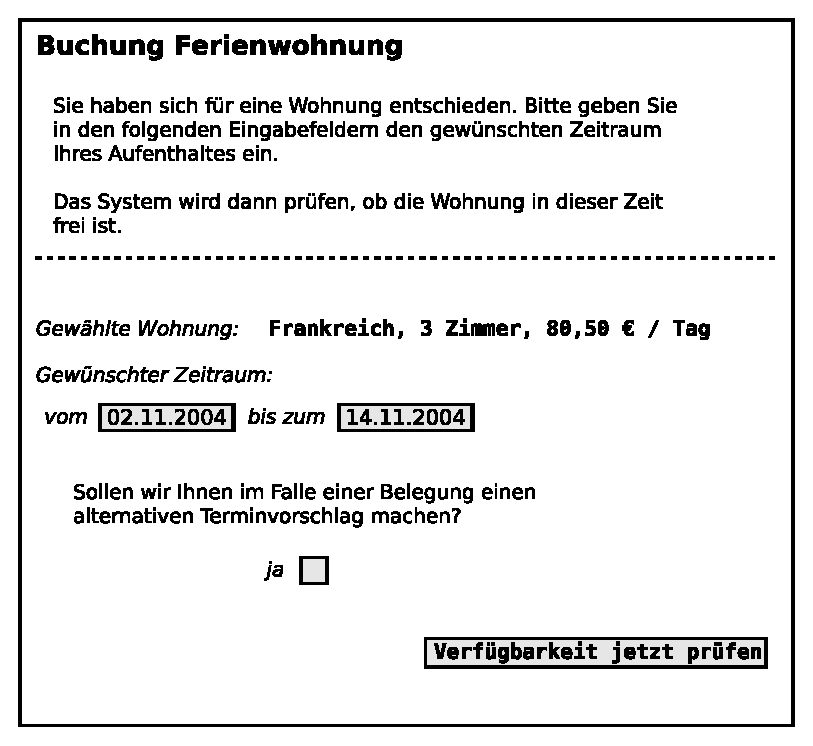
\includegraphics[width=0.75\textwidth]{images/screen_buchung.eps}
	\caption{Layoutbeispiel: Buchung einer Ferienwohnung}
	\label{fig:screen_buchung}
\end{figure}

\subsection{Datenschutzkonzept}
\subsubsection{Zugriffsberechtigte}
Aus dem Use-Case-Diagramm (\ref{fig:usecasediag}) lassen sich folgende Benutzer- bzw. Benutzergruppen ableiten:

\begin{itemize}
    \item Kunde (entspricht Datenbankuser \texttt{dbsys01})
    \item Interessent (entspricht Datenbankuser \texttt{dbsys33})
    \item Vermieter (entspricht Datenbankuser \texttt{dbsys02})
    \item Betreiber (entspricht Datenbankuser \texttt{dbsys34})
\end{itemize}

\subsubsection{Zugriffsrechte}
Ebenfalls dem Use-Case-Diagramm (\ref{fig:usecasediag}) entnommen werden k�nnen die ben�tigten Zugriffsrechte,
welche in der folgenden Matrix aufgef�hrt sind.
(Zugriffsrechte = \{\textbf{r}ead, \textbf{w}rite, \textbf{d}elete\})

\begin{table}[htbp]
	\centering
		\begin{tabular}{@{}l|*{4}{c}}
			\toprule
			\multicolumn{1}{l}{\bfseries{Relation/Objekt}} & \multicolumn{4}{c}{\bfseries{Subjekt}} \\
			 & Interessent & Kunde & Vermieter & Betreiber \\			
			\midrule
			Kunde					&		& r,w & r 		& r,w,d \\
			Buchung				&		& r,w	& r 		& r,w,d \\
			Rechnung			&		& r		& r 		& r,w,d \\
			Ferienwohnung & r & r		& r,w,d	& r,w,d \\
			Land					& r & r		& r 		& r,w,d \\
			Fluglinie			& r & r		& r,w,d & r,w,d \\
			Entfernung		& r & r		& r,w,d & r,w,d \\
			Attraktion		& r & r		& r,w,d & r,w,d \\
			\addlinespace
			\bottomrule
		\end{tabular}
	\caption{Zugriffsrechte}
	\label{tab:Zugriffsrechte}
\end{table}

Es wurden lediglich Zugriffsrechte f�r \textit{komplette Tabellen} verwendet, nicht f�r einzelne
Spalten. Daraus folgt, dass z.B. f�r die Tabelle "`Kunde"' keine differenzierten Rechte existieren,
die den Zugriff auf Kundendaten nur dem dazugeh�rigen Kunden erlauben. 

Dazu m�sste zu jedem Kunden ein Datenbankuser angelegt werden, dem dann per 
speziellem \texttt{VIEW} Zugriff auf "`seine"' Daten gew�hrt w�rden k�nnte.

\newpage

\subsection{Erweitertes ER-Modell}
Aus den Systemanforderungen wird das konzeptionelle Datenbank-Design in Form folgenden ER-Modelles entwickelt.

\begin{figure}[H]
	\centering
		\input eerm
	\caption{EERM}
	\label{fig:eerm}
\end{figure}

\section{Implementierung}

\subsection{Relationen}
Durch Transformation des ER-Modells erh�lt man die nachstehenden flachen Relationen.

\begin{itemize}
    \item Attraktion = (\{ {\em AttraktionNr}, Name, Typ, Beschrieb, Landcode \})
    \item Bild = (\{ {\em BildNr}, Pfad, FerienwohnungNr \})
    \item Buchung = (\{ {\em BuchungNr}, Rechnungsdatum, von, bis, KundenNr, FerienwohnungNr \})
    \item Entfernung = (\{ km, FerienwohnungNr, AttraktionNr \})
    \item Ferienwohnung = (\{ {\em FerienwohnungNr}, AnzahlZimmer, Groesse, Preis, Landcode, hatSauna, hatSchwimmbad \})
    \item Fluglinie = (\{ {\em FluglinieNr}, Name \})
    \item Fluglinie\_Land = (\{ FluglinieNr, Landcode \})
    \item Kunde = (\{ {\em KundeNr}, Vorname, Nachname, PLZ, Stadt, Strasse, HausNr, BLZ, KontoNr, Landcode \})
    \item Land = (\{ {\em Landcode}, Name \})
\end{itemize}

\normalem
{\em Hinweis:} Hier sind bereits die nachtr�glich eingef�gten Surrogatschl�ssel (bspw. "`FerienwohnungNr"' in der Relation Ferienwohnung) aufgef�hrt, welche im ER-Modell noch nicht erscheinen.

\subsection{Datenbank}

\subsubsection{Anlegen von Tabellen, CREATE}
\lstinputlisting[language=SQL]{../create_tables.sql}

\subsubsection{Zugriffsrechte, GRANT}
\lstinputlisting[language=SQL]{../privileges.sql}

\subsubsection{Datenbef�llung, INSERT}
\lstinputlisting[language=SQL]{../data.sql}

\subsubsection{Abfragen, SELECT}
Nachfolgende SELECT-Abfragen sollen die Korrektheit des Datenmodells verifizieren.

Sprachlich l�sst sich das Ergebnis der ersten Abfrage wie folgt formulieren: "`Welche Ferienwohnungen
in der Schweiz mit Sauna sind in der Zeit vom 01.11.2004 bis 21.11.2004 noch frei?"'

\lstset{language=SQL}
\begin{lstlisting}[caption={SELECT-Befehl 1}]
SELECT f.fwnr, b.von, b.bis
FROM ferienwohnung f
LEFT OUTER JOIN buchung b
ON ( b.fwnr = f.fwnr )
WHERE
(
  ( b.von < '2004-11-01' AND b.bis < '2004-11-21' )
  OR 
  ( b.von > '2004-11-01' AND b.bis > '2004-11-21' )
  OR 
  ( b.bunr IS NULL )
)
AND f.landcode = 'ch'
AND f.hat_sauna = 1;

# Ergebnis:

      FWNR  VON        BIS
---------- --------- ---------
          6 22-FEB-04  05-MAR-04
\end{lstlisting}

"`Welche Ferienwohnungen in Frankreich sind h�chstens 100km von Disneyland entfernt?"'

\begin{lstlisting}[caption={SELECT-Befehl 2}]
SELECT f.fwnr,f.land,e.km,e.atnr
FROM ferienwohnung f
JOIN entfernung e
ON (f.fwnr = e.fwnr)
WHERE e.atnr = 2
AND f.landcode = 'fr'
AND e.km <= 100;

# Ergebnis:
      FWNR  LAND          KM        ATNR
---------- ---- ----------  ---------- 
          3 fr          60.4            2
          4 fr          45.5            2
\end{lstlisting}

"`Wieviele Reservierungen gibt es f�r die einzelnen L�nder?"'
\begin{lstlisting}[caption={SELECT-Befehl 3}]
SELECT f.landcode,COUNT(*) 
FROM ferienwohnung f
JOIN buchung b
ON (f.fwnr = b.fwnr)
JOIN land l
ON (l.landcode = f.landcode)
GROUP BY f.landcode;

# Ergebnis:
LAND   COUNT(*)
---- ----------
ch             1
de             2
fr             1
it             1
\end{lstlisting}

%%% end main document
%%%
%%%%%%%%%%%%%%%%%%%%%%%%%%%%%%%%%%%%%%%%%%%%%%%%%%%%%%%%%%%%%%%%%%%%%%%%%%%%%%%%

%\appendix  %% include it, if something (bibliography, index, ...) follows below

%%%%%%%%%%%%%%%%%%%%%%%%%%%%%%%%%%%%%%%%%%%%%%%%%%%%%%%%%%%%%%%%%%%%%%%%%%%%%%%%
%%%
%%% bibliography
%%%
%%% available styles: abbrv, acm, alpha, apalike, ieeetr, plain, siam, unsrt
%%%
% \bibliographystyle{plain}

%%% name of the bibliography file without .bib
%%% e.g.: literatur.bib -> \bibliography{literatur}
% \bibliography{FIXXME}

\end{document}
%%% }}}
%%% END OF FILE
%%%%%%%%%%%%%%%%%%%%%%%%%%%%%%%%%%%%%%%%%%%%%%%%%%%%%%%%%%%%%%%%%%%%%%%%%%%%%%%%
%%% Notice!
%%% This file uses the outline-mode of emacs and the foldmethod of Vim.
%%% Press 'zi' to unfold the file in Vim.
%%% See ':help folding' for more information.
%%%%%%%%%%%%%%%%%%%%%%%%%%%%%%%%%%%%%%%%%%%%%%%%%%%%%%%%%%%%%%%%%%%%%%%%%%%%%%%%
%% Local Variables:
%% mode: outline-minor
%% OPToutline-regexp: "%% .*"
%% OPTeval: (hide-body)
%% emerge-set-combine-versions-template: "%a\n%b\n"
%% End:
%% vim:foldmethod=marker
